\section{YCSB Validation: Supplementary Details}
\label{sec:appendix-ycsb}

This section supplements the experimental setup and extended results from \S\ref{sec:eval-ycsb}.

\paragraph{Data scale and segment size skew}
Table~\ref{tab:c6-trace-density} summarizes the segment size distribution under YCSB Zipfian ($\alpha{=}0.99$) at three data-scale tiers. As the number of records grows from 20M to $2{\times}10^9$, the gap between the hottest and coldest segments widens to nearly $50\times$, reflecting the typical structure of Zipfian skew under range partitioning.

\paragraph{Fault families and parameterization}
The injection methods and severity sweep parameters for the four fault families are given in Table~\ref{tab:appendix-c6-faults}. Bimodal and Drift-shaped target concentrated patterns: the former drops a fixed fraction of keys within a contiguous window, while the latter concentrates additive discrepancies on the hottest segments, modelling replica lag under Zipfian skew. Uniform Diffuse and Weighted Diffuse both target diffuse patterns; Uniform Diffuse samples non-empty segments uniformly, whereas Weighted Diffuse samples dropped keys with probability proportional to each segment's record count, simulating independent per-record loss.


\begin{table*}[!htbp]
\centering
\small
\begin{tabular}{lp{0.76\textwidth}}
\toprule
Fault family & Parameterization \\
\midrule
\textbf{Bimodal} & Proportional key dropping within a contiguous 3-segment window, $r_{\text{drop}} \in \{0.05, 0.1, 0.2, 0.5\}$. \\
\makecell[tl]{\textbf{Drift-}  \textbf{shaped}} & Additive discrepancies concentrated on the hottest segments ($r_{\text{add}}{=}0.005$), modelling replica-lag under skew. \\
\midrule
\makecell[tl]{\textbf{Weighted}  \textbf{Diffuse}} & Global random key dropping, with dropped keys sampled with probability proportional to each segment's record count; $r_{\text{drop}} \in \{0.001, 0.003, 0.01, 0.03\}$. This simulates independent per-record loss under segment-size skew. \\
\makecell[tl]{\textbf{Uniform}  \textbf{Diffuse}} & Global random key dropping over non-empty segments with equal probability; $r_{\text{drop}} \in \{0.001, 0.003, 0.01, 0.03\}$.  \\
\bottomrule
\end{tabular}
\caption{Fault families and their parameterization (main text \S\ref{sec:eval-ycsb}).}
\label{tab:appendix-c6-faults}
\end{table*}

\paragraph{Sizing accuracy}
Drift-shaped is the most demanding fault family for sizing robustness, as it combines segment-size skew with a workload-shaped concentration of discrepancies in hot segments. With the Bessel correction applied, the median $|\mathrm{rel\_err\_scaled}|$ of the de-drifted estimator converges to approximately 1\% across all three data-scale tiers, matching the accuracy observed under the uniform settings of \S\ref{sec:eval-dedrift}. Per-tier values are reported in Table~\ref{tab:c6-sizing}.

\begin{table}[!htbp]
\centering
\small
\begin{tabular}{lrrr}
\toprule
Density tier & Records & seg size p50 & p99 \\
\midrule
Light   & 20M  & 35    & 1{,}689 \\
Medium  & 200M & 349   & 16{,}730 \\
Heavy   & 2B   & 3{,}487 & 167{,}675 \\
\bottomrule
\end{tabular}
\caption{The three density tiers correspond to the segment fill states of the same YCSB Zipfian workload at different data volumes.}
\label{tab:c6-trace-density}
\end{table}


\begin{table}[!htbp]
\centering
\small
\begin{tabular}{lcccc}
\toprule
Density & dedrift med & dedrift p90 & raw med & raw p90 \\
\midrule
Light  & 0.0077 & 0.0175 & 0.0397 & 0.0614 \\
Medium & 0.0141 & 0.0280 & 0.0313 & 0.0431 \\
Heavy  & 0.0096 & 0.0225 & 0.0384 & 0.0516 \\
\bottomrule
\end{tabular}
\caption{Sizing error ($|\mathrm{rel\_err\_scaled}|$) under Drift-shaped faults. The de-drift estimator outperforms the raw baseline across all three data-scale tiers.}
\label{tab:c6-sizing}
\end{table}




\begin{figure*}[!htbp]
\centering
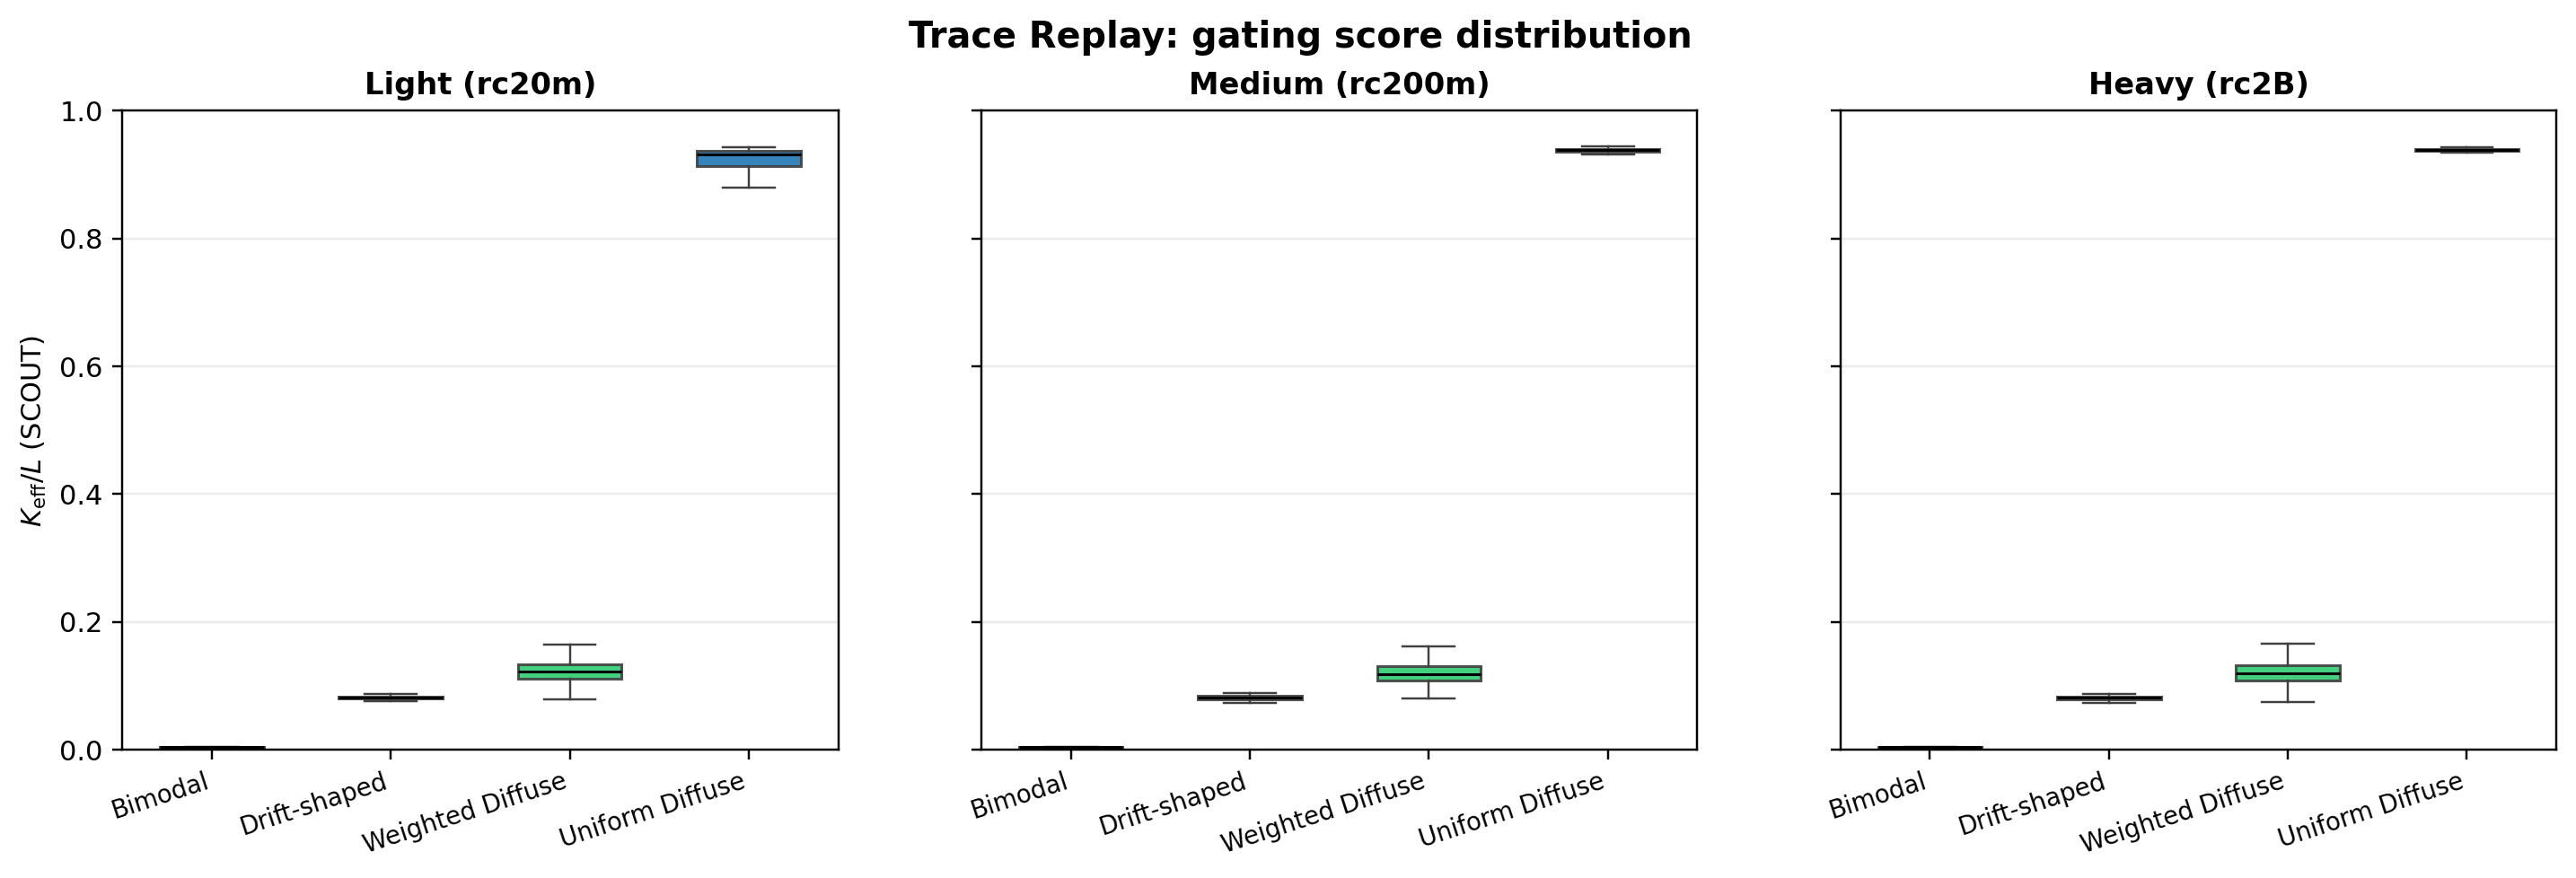
\includegraphics[width=0.8\linewidth]{figures/fig_c5b_b_gating_keff_boxplot.png}
\caption{Distribution of $K_{\text{eff}}/L$ under YCSB-driven workloads. Each panel corresponds to one data-scale tier; the four box-plot groups correspond to the four fault families.}
\label{fig:c6-gating}
\end{figure*}

\paragraph{Weighted Diffuse and the head-triage interpretation}
\label{sec:appendix-ycsb-weighted}
Weighted Diffuse is deferred from the main text because the
standard $\texttt{recall\_big}$ metric does not apply
directly: unlike Bimodal and Drift-shaped, whose injection
geometry provides a natural heavy-segment set, Weighted
Diffuse spreads discrepancies across nearly all segments
while concentrating most diff mass in a small head
(the top~285 segments, $0.3\%$ of~$P$, account for 50\%
of total diff mass). We therefore define a mass-based head
target $H_{0.5}$---the minimum prefix covering 50\% of diff
mass when segments are sorted by discrepancy count---and
report two companion metrics: \emph{head recall}
($|C \cap H_{0.5}|/|H_{0.5}|$), the fraction of heavy
segments captured by the candidate set, and \emph{head mass
coverage} ($\sum_{p\in C\cap H_{0.5}} d_p / \sum_{p\in
H_{0.5}} d_p$), the share of their discrepancy mass that is
captured. The latter is typically higher because top-ranked
segments each contribute disproportionately more mass.

Table~\ref{tab:c6-weighted-head} summarizes the resulting
operating points.  At a candidate fraction of approximately
$0.009$ (i.e., scanning less than 1\% of all segments),
SCOUT already covers roughly 83\% of the head mass; at
approximately $0.028$, coverage rises to about 90\%.
These operating points are nearly invariant across the three
data-scale tiers, consistent with the stability observed for
the other families in the main text.

\begin{table}[!htbp]
\centering
\small
\setlength{\tabcolsep}{3pt}
\begin{tabular}{rcccccc}
\toprule
 & \multicolumn{3}{c}{head recall} & \multicolumn{3}{c}{head mass cov.} \\
\cmidrule(lr){2-4}\cmidrule(lr){5-7}
\texttt{cand\_frac} & Light & Medium & Heavy & Light & Medium & Heavy \\
\midrule
${\sim}10^{-5}$  & 0.004 & 0.004 & 0.004 & 0.15 & 0.16 & 0.16 \\
${\sim}0.009$    & 0.40  & 0.39  & 0.40  & 0.83 & 0.83 & 0.84 \\
${\sim}0.028$    & 0.61  & 0.60  & 0.60  & 0.90 & 0.90 & 0.90 \\
${\sim}0.127$    & 0.88  & 0.89  & 0.88  & 0.97 & 0.98 & 0.98 \\
\bottomrule
\end{tabular}
\caption{Weighted Diffuse head-triage operating points
  (SCOUT, $H_{0.5}$ target). Values are representative
  averaged across four severity levels 
  ($r_{\text{drop}}$).}
\label{tab:c6-weighted-head}
\end{table}

